\chapter{Results and Discussion}
\label{chapter:Results and Discussion}



% Here starts the thesis with an introduction. Please use nice latex and bibtex entries \cite{latex}. Do not spend time on formating your thesis, but on its content. 
 
\section{Results and Discussion}
In this chapter, we evaluate the proposed algorithm using real data acquire using 
the camera rig system shown in \ref{ fig:rigsetup} and compare result with different 
approaches \todo{ define approaches}

\begin{figure}
\begin{adjustwidth}{-1in}{-1in} 
\centering     %%% not \center
\subfigure[Figure A]{\label{fig:a}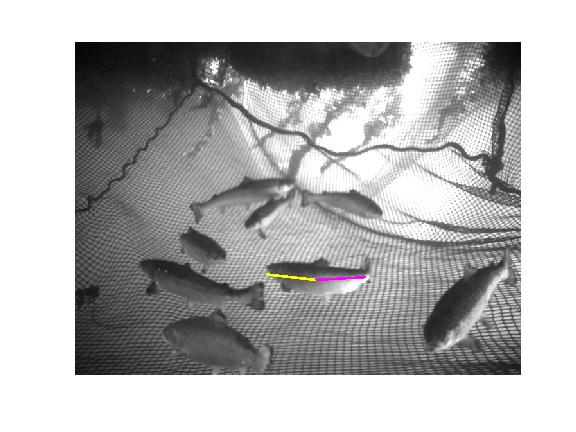
\includegraphics[width=50mm]{res/ram/3/im0218.jpg}}
\subfigure[Figure B]{\label{fig:b}\includegraphics[width=50mm]{res/ram/3/im0219.jpg}}
\subfigure[Figure C]{\label{fig:c}\includegraphics[width=50mm]{res/ram/3/im0220.jpg}}
\subfigure[Figure D]{\label{fig:d}\includegraphics[width=50mm]{res/ram/3/im0221.jpg}} \\
\subfigure[Figure A]{\label{fig:a}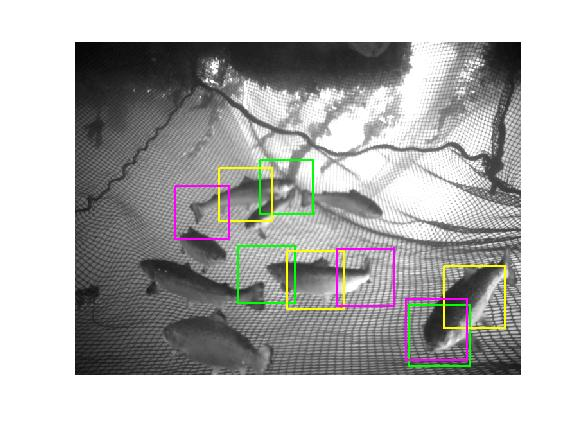
\includegraphics[width=50mm]{res/ram/3/im0218_m.jpg}}
\subfigure[Figure B]{\label{fig:b}\includegraphics[width=50mm]{res/ram/3/im0219_m.jpg}}
\subfigure[Figure C]{\label{fig:c}\includegraphics[width=50mm]{res/ram/3/im0220_m.jpg}}
\subfigure[Figure D]{\label{fig:d}\includegraphics[width=50mm]{res/ram/3/im0221_m.jpg}}
\caption{my caption}
\end{adjustwidth}
\end{figure}


\begin{figure}
\begin{adjustwidth}{-1in}{-1in} 
\centering     %%% not \center
\subfigure[Figure A]{\label{fig:a}\includegraphics[width=50mm]{res/ram/5/im0219.jpg}}
\subfigure[Figure B]{\label{fig:b}\includegraphics[width=50mm]{res/ram/5/im0220.jpg}}
\subfigure[Figure C]{\label{fig:c}\includegraphics[width=50mm]{res/ram/5/im0221.jpg}}
\subfigure[Figure D]{\label{fig:d}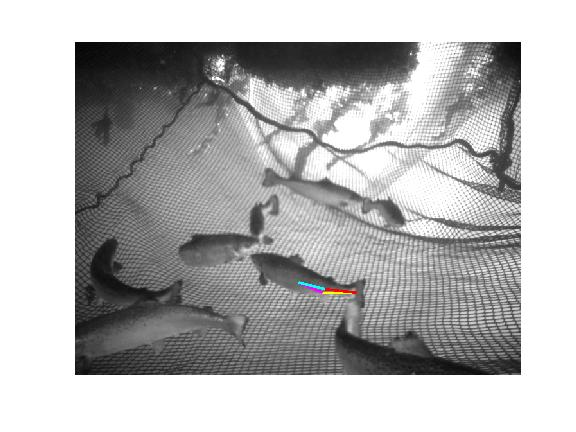
\includegraphics[width=50mm]{res/ram/5/im0222.jpg}} \\
\subfigure[Figure A]{\label{fig:a}\includegraphics[width=50mm]{res/ram/5/im0219_m.jpg}}
\subfigure[Figure B]{\label{fig:b}\includegraphics[width=50mm]{res/ram/5/im0220_m.jpg}}
\subfigure[Figure C]{\label{fig:c}\includegraphics[width=50mm]{res/ram/5/im0221_m.jpg}}
\subfigure[Figure D]{\label{fig:d}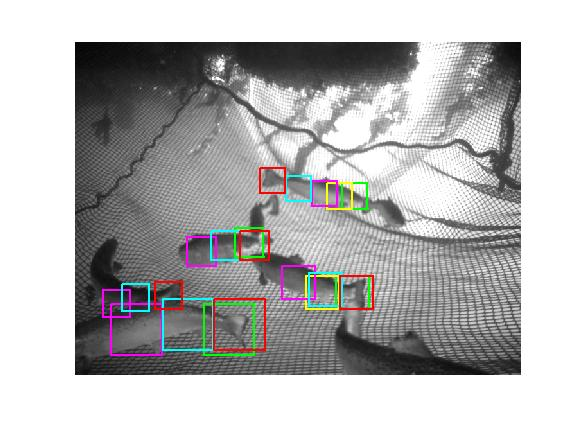
\includegraphics[width=50mm]{res/ram/5/im0222_m.jpg}}
\caption{my caption}
\end{adjustwidth}
\end{figure}

\begin{tabular}{ | l | l | r | }
  \hline\noalign{\smallskip}
  \multicolumn{2}{c}{Item} \\
  \cline{1-2}\noalign{\smallskip}
  Animal & Description & Price (\$) \\
  \noalign{\smallskip}\hline\noalign{\smallskip}
  Gnat  & per gram & 13.65 \\
        & each     &  0.01 \\
  Gnu   & stuffed  & 92.50 \\
  Emu   & stuffed  & 33.33 \\
  Armadillo & frozen & 8.99 \\
  \noalign{\smallskip}\hline
\end{tabular}


\section{Discussion}


% \section{Next Section}
% There is no need for a latex introduction since there is plenty of literature out there.
